\chapter{Elettrostatica}

\section{Legge di Coulomb}
  
La forza $\vec{F}_{12}$ esercitata da $q_1$ su $q_2$ è uguale in modulo e opposta in direzione alla forza $\vec{F}_{21}$ esercitata da $q_2$ su $q_1$.
    \begin{displaymath}
    	|\vec{F}_{12}| = |\vec{F}_{21}| = k_e \cdot \frac{q_1 \cdot q_2}{r^2}
    \end{displaymath}
Nel caso in cui le due cariche abbiano lo \textbf{stesso segno}, la forza è attrattiva (le due cariche si attraggono):
	\begin{figure}[h!]
      \centering
      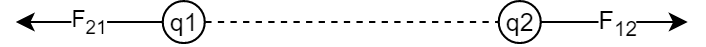
\includegraphics[scale=0.4]{esempio1}
  \end{figure}
  	\begin{displaymath}\begin{aligned}
    	\vec{F}_{12} = - k_e \cdot \frac{q_1 \cdot q_2}{r^2} \cdot \vec{u}_r\\
        \vec{F}_{21} = k_e \cdot \frac{q_1 \cdot q_2}{r^2} \cdot \vec{u}_r
    \end{aligned}\end{displaymath}
Nel caso in cui le due cariche abbiano \textbf{segno opposto}, la forza è repulsiva (le due cariche si respingono):
    \begin{figure}[h!]
    	\centering
        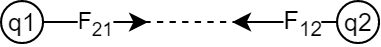
\includegraphics[scale=0.4]{esempio2.png}
	\end{figure}
    \begin{displaymath}\begin{aligned}
        \vec{F}_{12} = k_e \cdot \frac{q_1 \cdot q_2}{r^2} \cdot \vec{u}_r\\
        \vec{F}_{21} = - k_e \cdot \frac{q_1 \cdot q_2}{r^2} \cdot \vec{u}_r
    \end{aligned}\end{displaymath}
    
\section{Principio di sovrapposizione}
In un sistema di $n$ cariche, volendo valutare la forza totale agente su una carica $q$, è necessario sommare le forze esercitate da ciascuna carica. Ciascuna di queste forze agisce come se fosse l'unica presente.
	\begin{displaymath}\begin{aligned}
		\vec{F} = \sum_{i=1}^n k_e \cdot \frac{q \cdot q_i}{r_i^2} \cdot \vec{u}_{r_i}
	\end{aligned}\end{displaymath}

\section{Campo elettrico}
Dato un sistema di $n$ cariche, su una carica di prova $q$, agisce un campo elettrico $\vec{E}$ dato da:
	\begin{displaymath}\begin{aligned}
		\vec{E} = \sum_{i=0}^n k_e \cdot \frac{q_i}{r_i^2}\vec{u}_{r_i}
	\end{aligned}\end{displaymath}
La forza agente su $q$ può essere espressa come:
	\begin{displaymath}
		\vec{F} = q \cdot \vec{E}
	\end{displaymath}
    
\section{Teorema di Gauss per il campo elettrico}
Il teorema di Gauss per il campo elettrico permette di calcolare il flusso del campo elettrico generato da una certa distribuzione di carica elettrica attraverso una superficie senza svolgere i calcoli prescritti dalla definizione di flusso.\\
Data una superficie chiusa $S$ contenente $n$ cariche elettriche (positive o negative), il flusso del campo elettrico (generato dalle cariche) attraverso tale superficie è uguale al rapporto tra carica totale contenuta nella superficie chiusa e la costante dielettrica $\epsilon$ del mezzo in cui si trovano le cariche ($\epsilon_0$ nel vuoto):
\begin{displaymath}
	\Phi_S(\vec{E}) = \frac{\sum_{i=1}^n q_i}{\epsilon_0}
\end{displaymath}

\subsection{Distribuzione lineare}
Una distribuzione uniforme lineare di carica (es. \textit{una sottile asticella carica}) di lunghezza $L$, con densità di carica lineare positiva uniformemente distribuita
$$\lambda = \frac{q}{L}$$
Dove $q$ rappresenta la carica totale di cui è dotata l'intera asticella.
    \begin{figure}[h!]
    	\centering
    	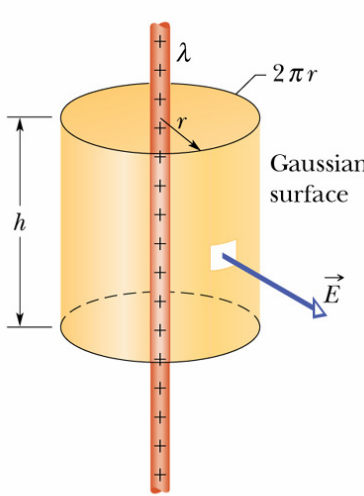
\includegraphics[scale=0.4]{esempio3.png}
    \end{figure}
Il campo elettrico $\vec{E}$ è perpendicolare alla superficie gaussiana:
	\begin{itemize}
    	\item{$\Phi(\vec{E})$ attraverso le basi è nullo.}
        \item{$\Phi(\vec{E})$ attraverso la superficie laterale è pari a $E \cdot (2 \cdot \pi \cdot r \cdot h)$.}
    \end{itemize}
Per il teorema di Gauss:
	\begin{displaymath}\begin{aligned}
		\epsilon_0 \cdot \Phi(\vec{E}) = q\\
        \epsilon_0 \cdot \int_S \vec{E} \cdot d\vec{A} = q\\
        \epsilon_0 \cdot E \cdot (2 \cdot \pi \cdot r \cdot h) = q = \lambda \cdot h\\
        \vec{E} = \frac{\lambda}{2 \cdot \epsilon_0 \cdot \pi \cdot r \cdot h}
	\end{aligned}\end{displaymath}
  
\subsection{Distribuzione piana}
Una distribuzione uniforme piana di carica, avente area $A$, è caratterizzata da una densità superficiale:
$$q = \sigma \cdot A$$ 
\begin{figure}[h!]
	\centering
	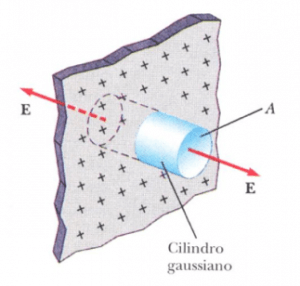
\includegraphics[scale=0.5]{esempio4.png}
\end{figure}
In una distribuzione di carica piana, la cui superficie 
Il campo elettrico $\vec{E}$ è perpendicolare alla superficie gaussiana:
	\begin{itemize}
    	\item{$\Phi(\vec{E})$ attraverso la superficie del cilindro è nullo.}
        \item{$\Phi(\vec{E})$ attraverso la le basi del cilindro è pari a $E \cdot A$, dove $A$ è l'area di una base.}
    \end{itemize}
Per il teorema di Gauss:
	\begin{displaymath}\begin{aligned}
		\epsilon_0 \cdot \Phi(\vec{E}) = q\\
        \epsilon_0 \cdot \int_S \vec{E} \cdot d\vec{A} = q\\
        \epsilon_0 \cdot (E\cdot A + E \cdot A) = q \cdot \sigma \cdot A\\
        2 \cdot \epsilon_0 \cdot E\cdot A = q = \sigma \cdot A\\
        E = \frac{\sigma}{2 \epsilon_0}
	\end{aligned}\end{displaymath}


\section{Energia elettrica}
\subsection{La forza elettrica è conservativa}
Posta una carica $Q$, ferma in un punto origine, calcoliamo il lavoro fatto dalla forza elettrica $\vec{F}$ per portare una carica $q_0$ da un punto iniziale $i(\vec{r}_i)$ a un punto $f(\vec{r}_f)$.
\begin{figure}[h!]
	\centering
	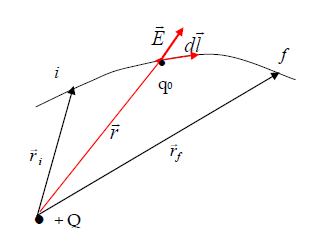
\includegraphics[scale=0.8]{lavoro1}
\end{figure}
\begin{displaymath}\begin{aligned}
\vec{E} = \frac{Q}{r^2} \cdot \vec{u}_r \qquad \qquad 
\vec{F} = q_0 \cdot \vec{E}\\
L = \int_i^f \vec{F} \cdot d\vec{l} = 
q_0 \cdot \int_i^f \vec{E} \cdot d\vec{l}=
k_e \cdot(q_0 \cdot Q) \cdot \int_i^f \frac{1}{r^2} \cdot \vec{u}_r \cdot d\vec{l} 
\end{aligned}\end{displaymath}
Osserviamo che 
\begin{displaymath}
\vec{u}_r = dl \cdot \cos{\theta} = dr
\end{displaymath}
Possiamo quindi scrivere:
\begin{displaymath}
L = k_e \cdot(q_0 \cdot Q) \cdot \int_i^f \frac{1}{r^2} \cdot \vec{u}_r \cdot d\vec{l}=k_e \cdot(q_0 \cdot Q) \cdot \left( \frac{1}{r_i} - \frac{1}{r_f}\right) = U(i)-U(f)
\end{displaymath}
Siamo riusciti a scrivere il lavoro della forza elettrica come una differenza di potenziali: ciò significa che la forza elettrica è conservativa.\\
Il lavoro della forza elettrica non dipende dal percorso, ma solo dalla posizione del punto iniziale e del punto finale.\\
Inoltre, il lavoro della forza elettrica lungo un percorso chiuso è nullo.

\subsection{Energia potenziale elettrica}
L'energia potenziale è l'inverso del lavoro compiuto dalla forza nello spostamento di una carica $q_0$ dal punto $A$ al punto $B$.
	\begin{displaymath}\begin{aligned}
		\Delta U = - L_{AB} =
        k_e\cdot q_1 \cdot q_0 \cdot  \left(\frac{1}{r_B} - \frac{1}{r_A}\right) = 
	\end{aligned}\end{displaymath}
Finora abbiamo parlato di variazione di energia potenziale tra due punti. Un'estensione del concetto porta alla definizione di energia potenziale in un singolo punto $b$, scegliendo un punto di riferimento $a$ e assegnando un valore di riferimento $U_a$ all'energia potenziale in quel punto.\\
Spesso conviene scegliere il punto $a$ di riferimento a distanza infinita, scegliendo $U_a = 0$ in quel punto.\\
Consideriamo il caso di una carica $q_1$ ferma nell'origine, e una carica $q_2$ che si sposta da $\vec{r}_a$ a $\vec{r}_b$
Se, in questo caso, $b$ rappresenta un generico punto di coordinata $r$:
	\begin{displaymath}
		U(r) = \frac{1}{4 \pi \cdot \epsilon_0}
		\cdot \frac{q_1 \cdot q_2}{r}
	\end{displaymath}


\subsection{Potenziale elettrico}
Sia $q_0$ una carica di prova in moto da $A$ a $B$, sotto l'azione di un campo elettrico $\vec{E}$.\\
Definiamo la differenza di potenziale (che sta all'energia potenziale elettrica come il campo elettrico sta alla forza di Coulomb):
	\begin{displaymath}\begin{aligned}
			\Delta V= \frac{\Delta U}{q_0} = -  \frac{L_{AB}}{q_0}
	\end{aligned}\end{displaymath}
Analogamente al calcolo dell'energia potenziale,  calcolare il potenziale in un punto $b$ è necessario prendere come riferimento il potenziale in un punto $a$.\\
\begin{displaymath}
	V(b) = k_e \cdot \frac{q}{r_b} + V_a
\end{displaymath}	
Solitamente, consideriamo come punto di riferimento un punto all'infinito, a cui attribuiamo il valore di potenziale zero.\\\\ 
Per calcolare il campo elettrico dato il potenziale è necessario l'operatore \textbf{gradiente}. L'operatore gradiente, applicato a una funzione scalare, restituisce un vettore avente come componenti le derivate parziali della funzione.
\begin{displaymath}
	\vec{E}(r) = - \vec{\nabla} V(r)=
\end{displaymath}

\section{Dipolo elettrico}
Un dipolo elettrico è un sistema composto da due cariche uguali, di segno opposto, poste a distanza $d$ lungo un asse $x$, che identifichiamo con il versore $\vec{u}_x$ .\\
Viene definito il \textbf{momento di dipolo} $\vec{p}$ come 
\begin{displaymath}
\vec{p} = q \cdot d \cdot \vec{u}_x
\end{displaymath}
\begin{figure}[h!]
	\centering
    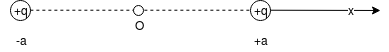
\includegraphics[scale=0.6]{DipoloElettrico}
\end{figure}


\subsection{Campo elettrico lungo l'asse del dipolo}
Il campo elettrico lungo l'asse del dipolo è pari alla somma dei campi elettrici generati da ciascuna carica.
\begin{displaymath}\begin{aligned}
	\vec{E}_+ = k_e \cdot \frac{q}{(r_x - a)^2} \cdot \vec{i}\\
    \vec{E}_- = - k_e \cdot \frac{q}{(r_x + a)^2} \cdot \vec{i}\\\\
    \vec{E} = k_e \cdot \left(\frac{q}{(r_x - a)^2} - \frac{q}{(r_x + a)^2} \right) \cdot \vec{i} = 
    k_e \cdot q \left( \frac{(r_x + a)^2 - (r_x - a)^2}{(r_x^2 - a^2)^2} \right) \cdot \vec{i} = \\
    k_e \cdot q \frac{r_x^2 + a^2 + 2 r_x a - r_x^2 +2 r_x a - a^2}{(r_x^2 - a^2)^2} \cdot \vec{i} = 
    k_e \cdot \frac{4 q r_x a}{(r_x^2 - a^2)^2} \cdot \vec{i}
\end{aligned}\end{displaymath}
Ricordando che $a = \frac{d}{2}$ e che $p = qd$:
\begin{displaymath}\begin{aligned}
	\vec{E} = k_e \cdot \frac{2p\cdot r_x}{(r_x^2 - (\frac{d}{2})^2)^2} \cdot \vec{i}    
\end{aligned}\end{displaymath}
Ha senso, in applicazioni reali considerare $r_x >>> d$, cioè misurare il campo elettrico a distanze molto maggiori della distanza tra le cariche del dipolo.
\begin{displaymath}
\vec{E} = k_e \cdot \frac{2 p r_x}{r_x^4} \cdot \vec{i} = k_e \cdot \frac{2p}{r_x^3} \cdot \vec{i}
\end{displaymath}

\subsection{Potenziale elettrico lungo l'asse del dipolo}
Il potenziale generato da una carica a una distanza $r$ è dato da:
\begin{displaymath}
	V(r) = k_e \cdot \frac{q}{r}
\end{displaymath}
Perciò, il potenziale del dipolo a una distanza $r_x$ è dato dalla somma dei potenziali dovuti a ciascuna carica (\textbf{additività dei potenziali}):
\begin{displaymath}\begin{aligned}
	V(r_x) = k_e \cdot \left( \frac{q}{r_x-a} - \frac{q}{r_x+a} \right) =
    k_e \cdot q \left( \frac{r_x + a - r_x + a}{r_x^2 -a^2} \right)=
    k_e \cdot q \cdot \frac{2a}{r_x^2-a^2}
\end{aligned}\end{displaymath}
Ricordando che $a = \frac{d}{2}$ e che $p = qd$:
\begin{displaymath}\begin{aligned}
	\vec{V} = k_e \cdot \frac{p}{r_x^2 - (\frac{d}{2})^2}    
\end{aligned}\end{displaymath}
Ha senso, in applicazioni reali considerare $r_x >>> d$, cioè misurare il potenziale a distanze molto maggiori della distanza tra le cariche del dipolo.
\begin{displaymath}
	\vec{V} = k_e \cdot \frac{p}{r_x^2}
\end{displaymath}
